\documentclass[authoryear]{elsarticle}
\usepackage{latexsym}
%\usepackage{rotate}
\usepackage{graphics}
\usepackage{amsmath}
\usepackage{amssymb}
\usepackage{comment}
\bibliographystyle{chicago}



\newcommand{\logit}{\mathrm{lgt}}
\newcommand{\I}{\mathrm{I}}
\newcommand{\E}{\mathrm{E}}
\newcommand{\p}{\mathrm{P}}
\newcommand{\e}{\mathrm{e}}
\renewcommand{\o}{\omega}
\newcommand{\vecm}{\mathrm{vec}}
\newcommand{\kp}{\otimes}
\newcommand{\diag}{\mathrm{diag}}
\newcommand{\cov}{\mathrm{cov}}
\newcommand{\eps}{\epsilon}
\newcommand{\ep}{\varepsilon}
\newcommand{\obdots}{\ddots}    % change this later
\newcommand{\Ex}{{\cal E}}
\newcommand{\Exd}{\Ex_d}
\newcommand{\Es}{\E_\phi}
\newcommand{\rat}{{\frac{c_{ij}}{c_{i,j-1}}}}
\newcommand{\rmu}{m}
\newcommand{\rsig}{\nu}
\newcommand{\fd}{\mu}
\newcommand{\tr}{\mathrm{tr}}
\newcommand{\cor}{\mathrm{cor}}
\newcommand{\bx}[1]{\ensuremath{\overline{#1}|}}
\newcommand{\an}[1]{\ensuremath{a_{\bx{#1}}}}

\newcommand{\bi}{\begin{itemize}}
\newcommand{\ei}{\end{itemize}}

\renewcommand{\i}{\item}
\newcommand{\sr}{\ensuremath{\mathrm{SRISK}}}
\newcommand{\cs}{\ensuremath{\mathrm{CS}}}
\newcommand{\cri}{\ensuremath{\mathrm{Crisis}}}
\newcommand{\var}{\ensuremath{\mathrm{VaR}}}
\newcommand{\covar}{\ensuremath{\mathrm{CoVaR}}}
\newcommand{\med}{\ensuremath{\mathrm{m}}}
\newcommand{\de}{\mathrm{d}}
\renewcommand{\v}{\ensuremath{\mathrm{v}_q}}
\newcommand{\m}{\ensuremath{\mathrm{m}}}
\newcommand{\tvar}{\ensuremath{\mathrm{TVaR}}}
\renewcommand{\c}{\ensuremath{\mathrm{CoVaR_q}}}
\renewcommand{\v}{\ensuremath{\mathrm{VaR}_q}}



\newcommand{\eref}[1]{(\ref{#1})}
\newcommand{\fref}[1]{Figure \ref{#1}}
\newcommand{\sref}[1]{\S\ref{#1}}
\newcommand{\tref}[1]{Table \ref{#1}}
\newcommand{\aref}[1]{Appendix \ref{#1}}




\newcommand{\cq}{\ , \qquad}
\renewcommand{\P}{\mathrm{P}}
\newcommand{\Q}{\mathrm{Q}}

\newcommand{\Vx}{{\cal V}}
\newcommand{\be}[1]{\begin{equation}\label{#1}}
\newcommand{\ee}{\end{equation}}




\begin{document}

% Title of paper
\title{Measuring background risk and systemic risk in finance}
% List of authors, with corresponding author marked by asterisk
\author{Piet de Jong,  Geoff Loudon and Weihao Choo \\[4pt]
% Author addresses
\textit{Department of Applied Finance and Actuarial Studies\\ Macquarie University, Sydney, NSW 2109.}
\\[2pt]
%E-mail address for correspondence
{piet.dejong@mq.edu.au}}

% Running headers of paper:
\markboth%
% First field is the short list of authors
{De Jong}
% Second field is the short title of the paper
{Systemic risk}

\begin{abstract}
This article refines, builds on, and extends  SRISK methodology recently proposed in the literature.  The refinement is to define SRISK in terms of a put on the Basel shortfall.   This  is built on by defining the background and systemic stress  of a firm as unconditional and departure from unconditional  expectation of the put, the latter when a hypothetical systemic stress is applied.  Systemic stress is defined in terms of a random variable and can take on variety of forms including alternative scenarios in usual stress testing as well stress driven by the interaction of variables.  Stressor random variables  are chosen by the practitioner.  Stressed expectations are linear, a sector systemic stress is naturally defined as linear in the firm specific systemic stress.      Application is made to Australian financial data. 
\end{abstract}

\maketitle

JEL classification
C15; E53; G21  (Needs to be filled out)

\section{Background}

Recent literature in the area of quantitative systemic stress measurement includes 
\cite{adrian2011covar},
\cite{acharya2012capital},
\cite{acharya2012measuring},
 \cite{brownlees2010volatility} and \cite{brownlees2015}.   The proposed research aims to extend and apply these techniques particularly in relation to the entities regulated by APRA.   Thus our  broad aim is to develop, implement and bring to bear recent developments in stress testing  on the aims of APRA and the CIFR targeted research areas.   (This needs much more commentary).

This study refines and develops recently proposed methods and applies the same to publicly available daily financial data for  the eight  Australian banks detailed in \tref{eightbanks} spanning the period from   3 April 2000 through to 1 December 2014.  The data is described in detail in \aref{data}.  Prices, adjusted for dividends are plotted in \fref{prices}.   Prices are combined with number of shares to derive total equity.    Total debt for each firm at each day is also collected.  (Should these be plotted?).

\begin{table}[htdp]
\label{banks}\caption{Major and minor Australian banks}\label{eightbanks}
\begin{center}
\begin{tabular}{l|l||l|l}
\hline
 \multicolumn{2}{c||}{major}& \multicolumn{2}{c}{minor}\\
 \hline
cba & Commonwealth Bank  & mqg & Macquarie \\
anz & Australia \& New Zealand  & boq & Bank of Queensland\\
nab & National Australia  & ben & Bendigo and Adelaide \\
wbc & Westpac & aba & Auswide \\
\hline
\end{tabular}
\end{center}
\end{table}%


\begin{figure}[htbp]
\begin{center}
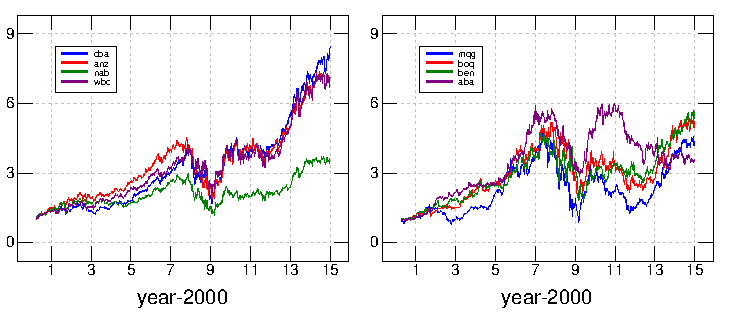
\includegraphics{figures/prices.pdf}
\caption{Stock  prices of four major (left panel) and four minor (right panel) Australian banks from early 2000 through to the end of 2014.  All prices normalised to start at 1.}
\label{prices}
\end{center}
\end{figure}


\section{Capital shortfall and leverage}

If $d_{it}$ and $w_{it}$ are the debt and equity of a firm $i$ at time $t$ and $\kappa$ is the capital requirement,  then the capital shortfall at time $t$ is 
\be{shortfall}
\kappa(d_{it}+w_{it}) - w_{it} = \kappa d_{it}  - (1-\kappa) w_{it} = \kappa d_{it}\left(1-\e^{-\ell_{it}}\right)\ ,
\ee
where 
$$
\ell_{it} \equiv  \ln\frac{\kappa d_{it}}{(1-\kappa)w_{it}}= \ln\frac{d_{it}}{w_{it}}+\logit(\kappa) \cq \logit(\kappa)\equiv \ln \frac{\kappa}{1-\kappa} \ .
$$
The quantity $\ell_{it}$ is called   adjusted log--leverage and $\ell_{it}>0$ implies capital shortfall \eref{shortfall} is positive.
Basel II assumes\footnote{See for example \cite{brownlees2015}.   The value of $\kappa$ can and is varied to test for sensitivity etc.} 
 $\kappa=0.08$ implying $\logit(\kappa)=-2.44$ and  $\ell_{it}$ is the actual log--leverage minus 2.44.   
As the actual  log leverage of a firm  increases to 2.44, the firm approaches a Basel breach. 

\fref{Bloglev} displays Basel log--leverages for the four major and four minor Australian banks listed in \tref{banks} on the first trading day of each month from January 2003  through to December 2014.  Note most banks are Basel compliant up to about 2008.

\begin{figure}[htbp]
\begin{center}
\label{Bloglev}
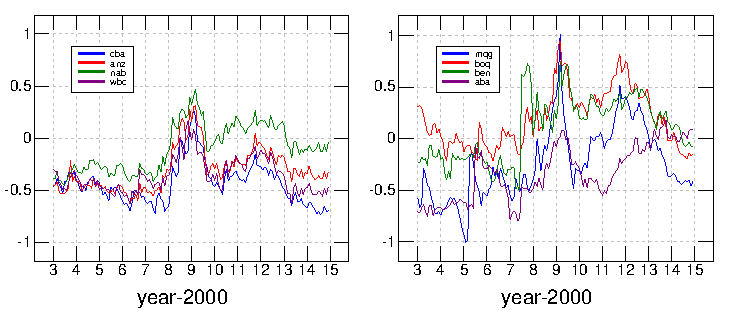
\includegraphics{figures/bloglev.pdf}
\caption{Adjusted log--leverages for four major (left panel) and four minor (right panel) Australian banks from the beginning of 2003 through to end of 2014.  All banks contravene the threshold (corresponding to the zero horizontal) around the start of 2009.}
\end{center}
\end{figure}


\section{Future capital shortfall}

Financial institutions and regulators are concerned with future Basel compliance and in assessing  the likelihood of a  future Basel breach.   Future compliance depends on the future return on equity.   Consider  firm $i$ at time  $t+h$ where $h>0$.  Then\footnote{In the further development $\e^\nu$ is the continuously compounded return and $\nu$  the  rate of return or log return.}
$$
\ell_{i,t+h} = \ln \frac{d_{i,t+h}}{w_{i,t+h}} +\logit(\kappa)= \ell_{it} -\nu_{it}\cq \nu_{it}\equiv \ln\frac{w_{i,t+h}}{w_{it}}  \ ,
$$
where it is assumed $d_{i,t+h}=d_{it}$.  Hence $\nu_{it}$ is the log return on equity over $(t,t+h)$.  The future return is unknown at time $t$ but its distribution may be  well understood.

The capital  shortfall  at time $t+h$ is,
\be{bs}
\kappa d_{it} |1-\e^{\nu_{it}-\ell_{it}}|^+\cq  |x|^+\equiv \max(0,x)\ . 
\ee
Thus shortfall \eref{bs} is a put on the return $\e^{\nu_{it}-\ell_{it}}$  with strike 1.  
The Basel  limit is reached at $t+h$ if $\nu_{it}=\ell_{it}$ and  breached  if
$\nu_{it}< \ell_{it}$.
A breach is  unlikely if $\ell_{it}$ is low i.e. either the log--leverage is low, or the  constant $\kappa$ in the calculation of $\ell_{it}$ is low.


If there is a breach, $\nu_{it}<\ell_{it}$, then the amount in \eref{bs} makes up for the shortfall.   This amount may be cold comfort to regulators as it leaves the firm in a precarious position, teetering on the edge of non--compliance.

Default put options similar to \eref{bs} have been discussed in the insurance literature as critical to an evaluation of a firm:  see for
example \citet{merton1977analytic}, \citet{doherty1986price}, \citet{cummins1988risk}, \citet{myers2001capital} and \citet{sherris2006solvency}.

To illustrate the setup, \fref{simulation}   displays two snapshot outputs from projections generated as described  in \aref{garchdcc}:  6000  simulated one month ahead projected returns for  CBA and the market, on  two dates: the first trading day in January 2009 and the first trading day in December 2014.    Both panels use the same horizontal and vertical scales.   Thus based on the available data at those two points in  time, policy makers and regulators faced entirely different projections based on the same time series model.   The scatter of dots are the forward simulations.  Note there is no lookahead bias as the model at each time point is based on the available data to that point in time.    The red horizontal line in each panel indicates the projected Basel limit:  any firm return less than the limit would constitute a Basel breach.   In the left panel there is little confidence that the Basel limit will be reached since it requires a return on equity approaching 20\% -- with confidence less than xxx the Basel standard will be breached.  In the right panel there is no chance of a Basel breach under any of the projected return on equity view -- the bank is ``safe."  
 
 The black dots in each panel indicate the actual outcome after one month.    In the left panel the outcome is a decline in both  the market and stock price.    In the right panel the returns are xxx and xxx.    Thus at the beginning of January  2009 the CBA bank was projected to be far from compliance in one month's time  while in December 2015 the one month projection is of complete compliance.  
 
 The two panels  display very different volatility and slopes.  These snapshots are used to compute systemic stress.  

\begin{figure}[htbp]
\begin{center}
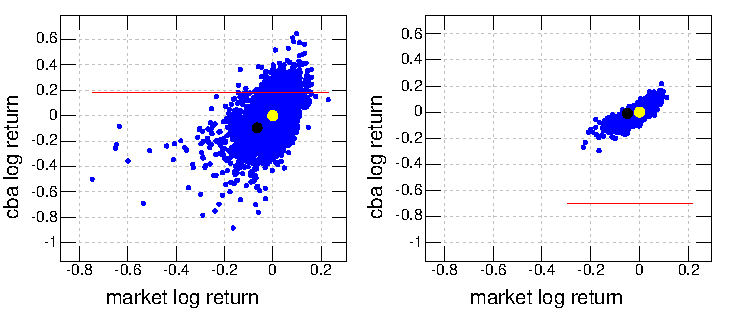
\includegraphics{figures/simulation.pdf}
\caption{Forecast bivariate distribution of one month forward rates of return   for CBA (vertical axis) and the market rate of return (horizontal axis) at start of January 2009 (left panel)  and December 2014 (right panel). Note scales in both panels are the same, the relatively large volatility in the left panel, and the left skew in the  marginal distributions.  Yellow and black dot in each panel indicate origin (0,0) and  realized forward  rate of return, respectively.   Red lines indicate Basel limit -- any firm return below the limit indicates a Basel breach given the bank leverage on the applicable date.}
\label{simulation}
\end{center}
\end{figure}




\section{Systemic risk -- SRISK}\label{srisk}

 \cite{brownlees2015} define  systemic risk (SRISK) for a group of firms  at time $t$ as
\be{esrisk}
\mathrm{SRISK}_t\equiv\kappa\sum_i d_{it}|1-\Es(\e^{\nu_{it}-\ell_{it}})|^+ \ ,
\ee
where  $\Es$ denotes  conditional expectation given a major general market downturn.  The proportionate contribution of firm $i$  to \eref{esrisk} is defined as the systemic risk in firm $i$  
 \be{sriskperc}
 \mathrm{SRISK}_{it}\equiv \frac{\pi_{it}|1-\Es(\e^{\nu_{it}-\ell_{it}})|^+}{\Ex_d\{|1-\Es(\e^{\nu_{it}-\ell_{it}})|^+\}}\cq \pi_{it}\equiv \frac{d_{it}}{d_t}\cq d_t\equiv \sum_i d_{it}\ , 
 \ee
where $\Ex_d$ denotes  debt weighted averaging at time $t$,  weighted averaging across firms $i$  using weights $\pi_{it}$.     Large $\mathrm{SRISK}_{it}$ indicates firm $i$ is systemically important: either because it holds a high proportion of the total debt, or it is unusually likely to breach the Basel capital requirement.  Expression \eref{sriskperc} depends on $\kappa$ through each of the $\ell_{it}$.  

Given a general market downturn, the values of the puts $|1-\Es(\e^{\nu_{it}-\ell_{it}})|^+$  in \eref{sriskperc} are known at time $t$:  there is no uncertainty except for possible  uncertainty in estimating the conditional  expected value.

Since
$$
|1-\Es(\e^{\nu_{it}-\ell_{it}})|^+ \le\Es(|1-\e^{\nu_{it}-\ell_{it}}|^+)\ ,
$$
with equality  if  $\nu_{it}-\ell_{it}$ is concentrated on the negative axis.  If  $\nu_{it}>\ell_{it}$  has positive probability then the  inequality is strict.   Further $\mathrm{SRISK}_{it}$ in \eref{sriskperc}   is zero whenever
$$
\Es(\e^{\nu_{it}})\le\e^{\ell_{it}}\ .
$$
This inequality typically holds even if the expectation conditions on an extreme market downturn. 

\section{Improved systemic risk measurement}

Following from \eref{bs}   define\footnote{Alternative terminology is the per unit capital shortfall put and the per unit expected capital shortfall.  For shortness we prefer the adjective Basel.  Note ``risk" here is not a probability but rather a measure of expected capital shortfall.} the  Basel put and  Basel risk of firm $i$ at time $t$ as
\be{put}
p_{it}\equiv |1-\e^{\nu_{it}-\ell_{it}}|^+\cq q_{it}\equiv \p(\nu_{it}\le \ell_{it})=\frac{\E(p_{it})}{\E(p_{it}|\nu_{it}\le \ell_{it})}\ ,
\ee
respectively, where $\E$ denotes unconditional expectation.  Note $0\le p_{it}\le 1$ with $p_{it}\rightarrow 0$ or 1 as $\nu_{it}\rightarrow\pm\infty$.
Further the Basel risk  $q_{it}$ increases as the distribution of $\nu_{it}$ moves to the left.  Both $\E(p_{it})$ and $q_{it}$ are thought of as probabilities of default with the former reflecting the whole distribution of $\nu_{it}$ given there is a default $\nu_{it}\le\ell_{it}$.


The total Basel put value  for firm  $i$ is   
$$
\kappa d_{it}\E(p_{it}) = \kappa d_{it}q_{it}\E(p_{it}|\nu_{it}\le \ell_{it})\ ,
$$
the cost of insuring firm $i$ does not breach the Basel standard.  In practice it may be appropriate to discount $p_{it}$ in \eref{put} by the interest rate over the period $(t,t+h)$ and value the put with risk neutral rather than normal expectation.       

The put $p_{it}$ is tradable since, given $\kappa$, it relies only on the present leverage and the future return $\nu_{it}$ on equity $w_{it}$.  Market participants can value the put in  the same way as any other put and use the contract to diversify risk.  Firms can buy puts in the market to hedge Basel default risk.    

However regulators will value the puts $p_{it}$ using a stressed, rather than risk neutral, expectation.   Stressed expectations correspond closely to conditional expectation given a system wide financial shock.    Regulators are concerned with the possibility of Basel breaches if such shocks occur and  have an  interest in monitoring stressed expectations.   In the extreme regulators can charge firms all or a  proportion of their stressed put values if there are implicit government bailout guarantees.


\section{Stressed expectation}

In the above development $\E$  is  unstressed expectation:  that is expectation that does not assume a stressful scenario.   A stressed expectation, denoted $\Es$, is a
linear combination of  expectations, each assuming some level of stress
\be{formula}
 \Es(p_{it}) \equiv \E\{\phi\E(p_{it}|\phi)\} = \E(\phi p_{it}) = \E(p_{it}) + \cov\{\E(p_{it}|\phi),\phi\}\ .
\ee 
Here $\phi\ge 0$ with $\E(\phi)=1$ is a stress factor or ``stressor,"  defining events impacting $p_{it}$  and serving as a basis for stress testing.  Thus stress $\phi$ changes the expected value $\E(p_{it})$ by the covariance between the conditional expectation $\E(p_{it}|\phi)$  and the stressor $\phi$.

The conditioning variable $\phi$  downplays or highlight different scenarios.  The conditioning events are scenarios of interest and  probabilistic weighting is according to the level of interest.  The first equality in \eref{formula}  from the definition of conditional probability \citep{whittle2000probability}.  The second equality follows from
$$
\cov(p_{it},\phi)=\cov\{\E(p_{it}|\phi),\phi\}\ .
$$
The covariance is zero whenever  $p_{it}$ is independent of $\phi$ which occurs if $\phi=1$.

The stressed expectation \eref{formula}  is the mean of $p_{it}$  using the  density
\be{post}
\int \phi f(p_{it},\phi)\de \phi= \E(\phi|p_{it})f(p_{it})\cq \int \phi f(p_{it},\phi)\de \phi\de p_{it} = \E(\phi) = 1\ 
\  ,
\ee
where $f$ denotes density.  
Any outcome $p_{it}$ such that $\E(\phi|p_{it})$ is large  is amplified and vice versa.   To a Bayesian the density in the left  expression of $\eref{post}$ is a posterior density given a prior $f(p_{it})$ and ``likelihood" $\E(\phi|p_{it})$: more importance is given to outcomes   $p_{it}$  where $\phi$ is expected to be large. 

\section{Background stress versus systemic stress}

The right hand side of \eref{formula} splits the stressed expectation $\Es(p_{it})$ into two components: 
\be{vsstress}
\Es(p_{it}) =\mu_{it}+s_{it}\cq 
 \mu_{it} \equiv \E(p_{it})=q_{it}\E(p_{it}|\nu_{it}\le \ell_{it}) \ ,
\ee
$$
s_{it} \equiv \cov\{\E(p_{it}|\phi),\phi\}\ , 
$$
called  the background stress  and systemic stress, respectively, in firm $i$ at time $t$.  Since both $\Es(p_{it})$ and $\E(p_{it})$ lie between 0 and 1 it follows both $\mu_{it}$ and $s_{it}$ lie between 0 and 1 and  are loosely interpreted as probabilities.  Further note 
$$
\E(p_{it}|\nu_{it}\le \ell_{it}) \approx \ell_{it}-\E(\nu_{it}|\nu_{it}\le \ell_{it})\ .
$$
and hence background risk decomposes into
$$
\mu_{it} \approx q_{it}\ell_{it} - q_{it}\E(\nu_{it}|\nu_{it}\le \ell_{it})
$$
(Weihao, do you think it is worthwhile to decompose the $s_{it}$ analogously in terms of a probability time a tail event?) 

The  term $\mu_{it}$  is called the background stress in firm $i$ and  reflects the log--leverage and the return volatility of firm $i$ at time $t$.  Background stress is unrelated to the stress factor $\phi$ and based on the unstressed distribution of the forward return $\nu_{it}$ and depends on the current view of the likely future progression of returns including their mean and volatility.     (Have to fill out discussion with how $mu_{it}$ measures the general uncertainty building up in the system with all  uncertainty  due to monitoring the system up to time $t$.)  Background stress is unrelated to the stress factor $\phi$.  Further
\be{mstress}
\mu_{it}=q_{it}\E(p_{it}|\nu_{it}\le \ell_{it})\ ,
\ee
where  $q_{it}$ is the Basel risk for  firm $i$  in the upcoming month,  while the second factor is the expected default size  (on a log scale)  if default occurs.
The probability $q_{it}$ depends on the  mean and volatility of daily returns at time $t$.

(*** unformed idea)   We can similarly decompose   (is this useful? -- Weihao can you look at this?)
$$
s_{it} = q_{\phi it}\E_\phi(p_{it}|\nu_{it}\le \ell_{it})-q_{it}\E(p_{it}|\nu_{it} \le \ell_{it})
$$      

Firm $i$ is at Basel default if $\ell_{it}=0$  and then  $q_{it}\approx 1/2$.   As  $\ell_{it}$ increases from zero,  one month ahead Basel default status  becomes more certain since $\nu_{it}\le \ell_{it}$ becomes more certain and $q_{it}$ increases to 1. 

   

  
   
\section{Systemic beta's}

The second, systemic stress component $s_{it}$ in  \eref{vsstress},  captures the financial impact of a  hypothetical system wide financial shock.   The stress $\phi$ is systemic as it is expected to affect all firms $i$.  Further $s_{it}$ is the estimated   increase in put values on account of  $\phi$.   Examples of stress factors are given in \sref{marketstress} and \sref{genstress}.
 

Writing  $\sigma_{\phi}$ as the standard deviation of $\phi$,  define the systemic beta of firm $i$ with respect to stress $\phi$ as
\be{zscore}
\beta_{it}\equiv \frac{s_{it}}{\sigma_\phi}
\ee
where  $\sigma_\phi$ is the standard deviation of $\phi$.   Thus $\beta_{it}$ is the systemic stress component in \eref{formula} standardised by $\sigma_\phi$ and
\be{zscore2}
\Es(p_{it})  = \mu_{it} + \beta_{it}\sigma_\phi\cq \E(p_{it}|\phi) \approx \mu_{it} + \beta_{it}\frac{\phi-1}{\sigma_\phi}\ .
\ee
The second, approximate, relationship is suggested from   $\cov(p_{it},\phi)/\sigma^2_\phi$ analogous to the regression coefficient of $p_{it}$ on $\phi$.

The expressions in \eref{zscore2} suggests two ways of  thinking about the  systemic beta's  $\beta_{it}$.   First, the left hand side equation shows systemic stress $\beta_{it}$ serves to shift the mean $\E(p_{it})$ of put prices  by, on average, $\sigma_\phi$.    The stress from $\phi$ is captured with $\sigma_\phi\beta_{it}$, the second term on the right of the first expression.   This term is called systemic stress and represents the addition to expected put prices if stress $\phi$ materialises.  

Systemic beta's are stated in terms of additions to the normal put price $\E(p_{it})$. Thus in an increasingly dire financial situation $\E(p_{it})$ will increase.   However  $\beta_{it}$ and the systemic stress measures the  change in current put values  under  further $\phi$--stress.  This varies from  \cite{brownlees2015} where $\mathrm{SRISK}_i$ does not distinguish between the current, possibly high, put prices $\E(p_{it})$ and the potential  increment due to potential stress.   Thus in an increasingly dire financial situation put prices are liable to increase on account of decreasing expected returns and increasing volatility.   However our definition of systemic stress using systemic beta's measures the further effect on account of potential extra stress imposed onto the system over and above the already existing stress.   Systemic beta's capture   ``marginal" effects.  

The second interpretation is based on  the right hand side approximation in \eref{zscore2} showing   the change in the  expected Basel put price if  $\sigma_\phi$ units of stress $\phi$ are applied.  The quantity $(\phi-1)/\sigma_\phi$ is thought of as a ``stress factor."   The stress factor has mean 0 and standard deviation 1 and is scaled by $\beta_{it}$ to yield the actual stress effect on  $p_{it}$.  Thus  $\beta_{it}$ is thought of a usual finance type ``beta" with respect to $\phi$.   Stress is measured in standardised units.  Units of stress take on different meaning depending on  $\phi$ as discussed below. The distribution of $\phi$ determines the distribution of the stress factor. If the stress factor is normally distributed then a stress effect more than doubling of the put value  occurs less than about $2.5\%$ of the time. 

      

The  monetary stress of a firm is 
$
d_{it}\beta_{it}
$
and represents the change in the monetary value of the Basel put  if stress, as captured with $\phi$, is applied. 

\section{Estimating background and systemic stress via simulation}

Stress $\mu_{it}$ and can be determined using simulation.   Suppose $(\phi^\o,p_{it}^\o)$ are pairs of stress and put values generated from a model: for example $\phi^\o$ may be zero unless there is a market drop below the $\alpha$--percentile in which case it is $1/\alpha$. 
Then 
\be{simulate}
\frac{1}{N}\sum_{\o=1}^N p_{it}^\o\rightarrow \mu_{it}\cq \frac{1}{N}\sum_{\o=1}^N (\phi^\o-1)p_{it}^\o\rightarrow s_{it} \cq N\rightarrow\infty\ ,
\ee
where $N$ is the simulation effort.  The approximation is increasingly accurate as $N$ becomes large.   More details are given in ...





\section{Stress based on  market return}\label{marketstress}
The setup is illustrated with  examples generalising and fine--tuning the approach of Engle.

\subsection{Market return below a percentile threshold} 

Suppose the stress event is a market return in the bottom $\alpha$--tail of the  market return distribution.   Then  $\phi(u)=1/\alpha$ for $u< \alpha$ and 0  otherwise and
$$
\Es(p_{it}) = \frac{1}{\alpha}\int_0^\alpha\E(p_{it}|u)\de u = \E(p_{it}|\nu_{mt}<\tau_{t}) \ .
$$
where $\tau_t$ cuts out $\alpha$ probability in the lower tail of the $\nu_{mt}$ distribution.   Further
$$
\mu_{it}\approx \frac{1}{N} \sum_\o p_{it}^\o \cq s_{it}   \approx  \frac{1}{N/\alpha} \sum_{u^\o_{mt}<1/\alpha}  p_{it}^\o\ .
$$
In the right hand sides $\o=1,\ldots,N$ denote $N$ simulations.  The approximations decrease with the simulation effort $N$.   The effective simulation effort is $N/\alpha$ and hence $\alpha$ small requires a  large effort. 

A fixed $\alpha$ cutoff  implies the actual threshold depends on the distribution and hence  on volatility and  time.  The actual threshold drop in the market $\tau_t=F_{mt}^-(\alpha)$, where $F_{mt}^-$ is the inverse distribution function of $\nu_{mt}$.  The volatility associated with the latter distribution is approximately $\sqrt{h}\sigma_{mt}$ where $\sigma_{mt}$ is current market volatility.   Regulators and practitioners  are well versed in working with VaR type calculations and hence a varying VaR type cutoff combining market volatility and stress is closely aligned to current practice. 


\subsection{Expected worst market return in $n$ identical scenarios} 
If $\phi(u)=n(1-u)^{n-1}$ then $\phi(u)\de u = \de\{1-(1-u)^n\}$ and 
$$
\Es(p_{it}) \equiv \E\{\phi\E(p_{it}|\phi)\} = \int_0^1\E(p_{it}|u)\de\{1-(1-u)^n\}\ .
$$
If $u$ is the market return percentile then  $1-(1-u)^n$ is the distribution of the worst percentile outcome in $n$ identical trials and hence the stressed expectation is that of the expected put price given the worst percentile market return in $n$ identical trials.  Further 
$$
s_{it}  \approx  \frac{1}{N} \sum_\o \{ n(1-u^\o_{mt})^{n-1}-1\}p_{it}^\o \ . 
$$
The effective simulation effort is $N/n$.
Simulated returns $\nu^\o_{mt}$ in the upper tail of the distribution  have percentiles $u^\o_{mt}\approx 1$ and hence for these market returns $(1-u^\o_{mt})^{n-1}$ is negligable and the associated simulated put $p_{it}^\omega$ is heavily downweighed.  

Note the contrast with the previous example where the bottom $\alpha$ proportion of simulated market returns are selected as the stressed sample. With the current specification for $\phi$,   every simulated put contributes to the stress computation, albeit with  different weights.


\subsection{Expected worst market return given a tail event}

The above two situations can be combined.   Suppose  $\phi(u)=c(0.05-u)^{19}$ for $u\le 0.05$ and 0 otherwise and where $c$ is such that $\phi(u)$ integrates to 1.  Then (this needs to be checked)
$$
\E(p_{it}) \approx \frac{1}{N/c}\sum_{u^\o_{mt}<1/20}  \left(u^\o_{mt}-\frac{1}{20}\right)^{20}p_{it}^\o\ .
$$
 Similar to the first example, the stressed sample picks up the bottom 5\% of market returns. The bottom 5\% of market returns is further stressed by  progressively downweighing returns as the percentile approaches 1/20.   Large simulation effort $N$ is required for a reasonable approximation since $N/c$ is the effective simulation size and $c$ is small.

\section{Simulating future capital shortfall and market return}

(maybe this should be merged with material elswhere).

The estimation of systemic beta's requires  projections of future capital shortfalls and future stressors.   As in \cite{brownlees2015} in this article projections are constructed  using time series models modelling the forward rates of return $\nu_{it}$ for firms $i$ and $\nu_{mt}$ for the market.   The market return is used as the stressor with different choices of the stress function $\phi$ modelling different stress scenarios.

The time series models used for projecting are stochastic volatility models based on the GARCH--DCC model of \cite{engle2002dynamic} summarised in \aref{garchdcc}.    The GARCH--DCC framework is only one possible implementation.   For example future return scenarios may be constructed in a more ad--hoc manner e.g. judiciously chosen scenarios decided on by regulators or policy makers.   The  systemic beta framework can be based on  any  generated  future  scenarios.

 
While the above discussion suggests, as obvious after the fact, that in December 2009 the CBA bank was under much stress.   However the above calculations do not actually reflect real stress.   In terms of the development of the previous sections the actual stress is beta given a stressor function $\phi$ and stressor variable.   In this case the stressor variable is the market return, on the horizontal axis in each panel.   Stress occurs if the market return is low.   In the left panel low market outcomes are likely to lead to sharply lower CBA bank returns, as compared to the right panel.   This is suggested by the slope of the scatter plots:  the left slope appears steeper than the right and hence any stress in the market -- in the sense of a market downturn is expected to lead to a larger drop in the CBA bank return in the left scenario as compared to the right scenario.   The magnitudes of the two responses depends on the stressor function.   In essence the stressor function formalises the notion as to what constitutes a ``big" drop.   If a big drop is the expected worst in 20 similar market scenarios then the stress in the left and right are xxx and xxx, respectively.   


\section{One month ahead forecast stress in individual financial institutions}

\fref{default} displays, in the top panels, the estimated $q_{it}$ one month ahead default probabilities for each major and minor Australian banks based on the projected one month ahead return distribution.   The  top left panel shows the first inclinations of default arose with NAB in early 2008 followed one month later by ANZ, and  a further few months later by WBC and CBA. 


Systemic stress is an expected  market return equal to the worst outcome in 12 identical months.  (Have to expand on this).
(Need much more commentary here)

 \begin{figure}[htbp]
\begin{center}
\label{default}
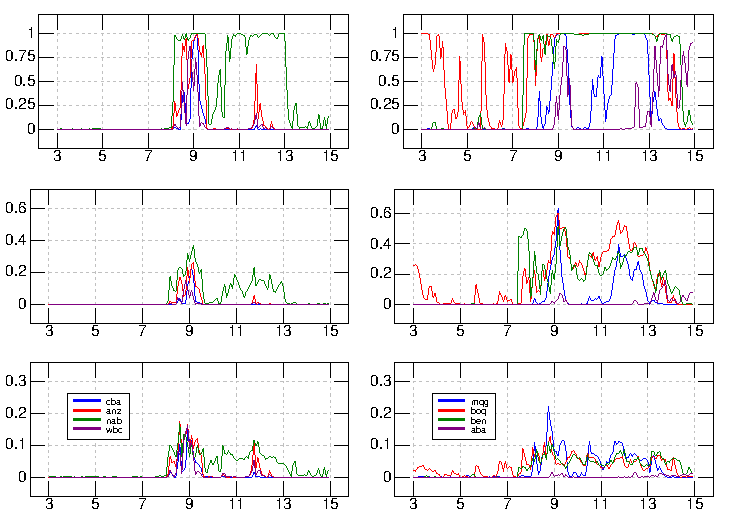
\includegraphics{figures/default.pdf}
\caption{Forecast one month ahead  Basel default probability (top panels), background stress (middle panels) and systemic stress (bottom panels) for  four major (left panel) and four minor (right panel)  banks from the beginning of 2003 through to end of 2014.  Note different scale on bottom two rows of panels.}
\end{center}
\end{figure}


\section{Average stress}

There are two ways of aggregating stress in the financial sector as a whole.  The first is to average, using debt weighted averaging, the put
\be{nsrisk}
\overline p_t \equiv \Exd(p_{it}) \cq \Es(\overline p_t)=\Exd\{\Es(p_{it})\} = \Exd(\mu_{it}+s_{it}) \equiv \overline\mu_{t}+\overline s_t
\ee
The put $\overline p_t$ in \eref{nsrisk} pays out zero if all firms meet the Basel requirement with payments increasing with the number of Basel breaches, the sizes of the breaches, and the relative debt sizes of the breaching firms.   Further $\overline p_t>0$  if and only if one or more firms breach the Basel standard.    The relation in \eref{nsrisk} follow since  $\Es$ and $\Exd$ are linear.   (Is $\overline q_t$ a useful concept?   Weihao can you look at this?) 

The monetary value  average  stress at time $t$ is the debt averaged  monetary firm stresses
$$
\kappa d_t\overline\mu_t = \kappa d_t\Exd(\mu_{it}) = \kappa\sum_i d_{it}\mu_{it}\cq \kappa d_t\overline s_t  = \kappa\sum_i d_{it}s_{it}\ . 
$$
Firm  $i$ contribution to for example systemic stress is   
$
\pi_{it}s_{it}/\overline s_t
$
which, when adding across firms, adds to 1.  Other contributions are calculated similarly.

Percentage contributions of firms to background and systemic stress are calculated as
$$
\frac{\pi_{it}\mu_{it}}{\overline \mu_t} \equiv \frac{\pi_{it}\mu_{it}}{\Ex_x(\mu_{it})}\cq \frac{\pi_{it}s_{it}}{\overline s_t} \equiv \frac{\pi_{it}s_{it}}{\Ex_x(s_{it})}\ .
$$
where $\pi_{it}\equiv d_{it}/d_t$ is the proportion of total debt held by firm $i$.   A ratio such as $s_{it}/\overline s_t$ compares the stress in firm $i$ to average stress but does not signal the importance of that firm to the system as a whole.  


\section{Total sector stress}

The debt weighed average system  put $\overline p_t\equiv\Ex_d(p_{it})$ is an average put and does not permit  diversification -- the  sharing of debt and equity across firms.   Sharing may not be possible in practice but the concept is useful for assessing the stability of the system as a whole.   This leads to the second way of aggregating stress in the financial sector as whole.

Write  $d_t$ and $w_t$ are total debt and equity in the financial sector, respectively:
$$
d_t \equiv \sum_i d_{it}\cq w_{it} \equiv \sum_i w_{it}\ .
$$
Then the   adjusted log leverage for the sector is  
$$
\ell_t \equiv  \ln \frac{d_t}{w_t} +\logit(\kappa) =  \ln \sum_i\frac{w_{it}}{w_t}\left(\frac{ d_{it}}{ w_{it}}\times \frac{\kappa}{1-\kappa}\right) = \ln \Ex_w(\e^{\ell_{it}}) \ ,
$$
where $\Ex_w$ denotes equity weighted averaging.  A system wide breach occurs at $t+h$ if
$
\nu_t < \ell_t
$
where $\nu_t$ is the forward rate of return on total equity $w_t$:
\be{ew}
 \nu_t =  \ln \frac{w_{t+h}}{w_t} = \ln\Ex_w\left(\frac{w_{i,t+h}}{w_{it}}\right) = \ln \Ex_w(\e^{\nu_{it}})\ . 
\ee
In terms of this notation the system Basel put  and Basel risk are defined similar to \eref{put}
$$
p_t\equiv |1-\e^{\nu_t-\ell_t}|^+\le \overline p_t\cq q_t\equiv \frac{\E(p_t)}{\E(p_{t}|\nu_t<\ell_t)}=\p(\nu_t\le \ell_t) \ .
$$
The inequality is proved in  \aref{proof}.  The  put $p_t$ pays 0 at time $t+h$ unless the sector as whole is in Basel default, occurring if $\nu_t  <  \ell_t$. Moving from $\overline p_t$ to $p_t$  allows for diversification:   low liquidity  in one firm is offset by high liquidity  in other  firms.  

\begin{figure}[htbp]
\begin{center}
\label{muqs}
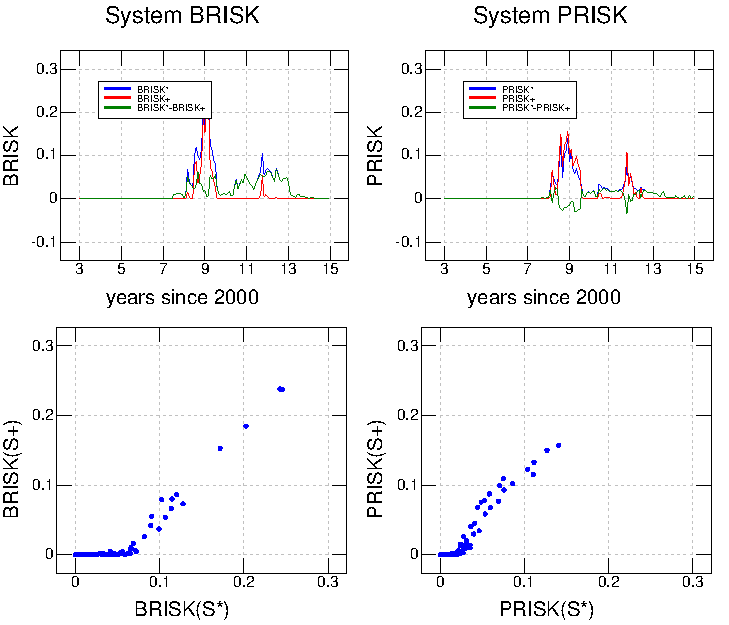
\includegraphics{figures/muqs.pdf}
\caption{Average  stresses and  total stresses.   Stress measurements are, left to right, $\mu$, $q$ and $s$, respectively.   The top row of panels measure for example (top left panel)  $\overline \mu_t$ and $\mu_t$ over time.    In the bottom row of panels  specific stresses are measured are against each other:  for example $\mu_t$ (vertical axis) versus $\overline\mu_t$ (horizontal axis).  In all cases there is no total stress until there is an appreciable level of average stress.  Systemic stress $\overline s_t$ appears to be the least diversifiable.}
\end{center}
\end{figure}

Similar  to \eref{zscore2}, total  stress is decomposed as 
\be{overall}
\Es(p_t) = \mu_t  + s_t\cq q_{t}=\P(\nu_t<\ell_t) \cq  s_t \equiv \cov\{\E(p_t|\phi),\phi\}\ .
\ee
termed the sector background  and systemic stress, respectively.   Further $q_t$ is the probability of  a sector Basel default with the second factor the expected size (on a log scale) of the default if there is a Basel default. 

System resilience aims to answer the question whether the system as a whole can absorb shocks.   The capacity to absorb relies on implicit merging.  When two firms merge the leverage of the resulting firm is less than that of the more highly leveraged firm.   The merged firm is more able to withstand return on equity shocks  unless negative shocks are more prone for the merged firm.   Similarly when many firms merge Basel puts for the conglomerate become less valuable.

Firms do not necessarily merge, even in dire financial circumstances.   Hence the mergers spoken of here are hypothetical.   From a regulators perspective, what would happen under a merger of all firms (or perhaps a group of firms) is nevertheless of interest.   A system as as a whole near Basel non--compliance is more threatening that one where a few firms are near Basel non--compliant but the system itself is well away from non--compliance.

System compliance  is partially monitored with the system put $p_t=\Exd(p_{it})$ and its stressed expectation $\Es(p_t)$.   The system put however simply monitors a debt weighted average of puts.   It gives no guidance as to how much risk can be diversified away.   Basing a put on system wide aggregated debt and equity and comparing the same to $p_t$  gives at least some guidance.

Possible additional issues to be discussed here
\bi
\i  Usually  $q_t<\overline q_t$ reflecting diversification benefits.   However this inequality is not guaranteed since ???
$$
\Ex_d\{\P (\nu_{it}\le \ell_{it})\} \ne  \P\{\Ex_d(\nu_{it})\le \Ex_d(\ell_{it})\}
$$
\i   Comparing say $\overline s_t/s_t$ or $(\overline\mu_t+\overline s_t/(\mu_t+s_t)$ etc.   What do each of these different measures illustrate? (System robustness)
\i   Percentage measures such as  $\pi_{it}s_{it}/s_t$,  or $\pi_{it}s_{it}/(s_t+\mu_t)$.
\i  System robustness such as 
\ei    










 
 \section{Further generalised stress functions}\label{genstress}
 
Practical results for the  construction of general stress functions $\phi$ are contained in the next three subsections.

 
 \subsection{Stress functions as  weighted linear combinations of tail events}
 

\cite{brownlees2015} define a systemic event as a market based downturn greater than a certain threshold and a systemic event  depends on the chosen threshold.   This arbitrariness is partially sidestepped by choosing a decreasing function $\phi=\phi(u_{mt})$ on the unit interval and noting 
\be{wave}
\E\{\phi\E(p_{it}|\phi)\} = -\E\{u\phi'(u)\E(p_{it}|u_{mt}\le u)\}\ .
\ee
The equivalence of the left and right hand sides of \eref{wave}  follows from 
$$
\int_0^1 \phi'(u)  \int_0^u \E(\nu_{it}|u_{mt})\de u_{mt}   \de u =\int_0^1\E(\nu_{it}|u_{mt})\int_{u_{mt}}^1  \phi'(u) \de u \de u_{mt}\ ,   
$$
provided $\phi(1)=0$.

Thus stressed expectations, stressed with a decreasing function of the market return, is equivalent to taking a weighted average of conditional lower tail expectations.  This result is used to circumvent an explicit choice for the market threshold, replacing it with  $\phi(u)$, an implicit  mixture of thresholds. 

\subsection{Scenario based stress testing}
 Stress events captured with $\phi$ and used  in \eref{zscore}  can be defined with respect any events, including a discrete number of scenarios labelled $k=1,2, \ldots$.   In this case 
$$
\Es(p_{it})= \sum_k \pi_k\phi_k\E(p_{it}|k)\cq \sum_k\pi_k\phi_k = \E(\phi) = 1 ,
$$
where $\phi_k$ is the weight assigned to scenario $\kappa$.   The $\pi_k\phi_k\ge 0$ are  modified  probabilities which weigh different scenarios according to level of interest.   For example in standard stress testing the $\phi_k$ are chosen such that significant weight is given to scenarios $\kappa$ causing high  firm distress.   The ``real world" probabilities $\pi_k$ are  usually ignored by  simply choosing  $\pi_k\phi_k$ to be of  required magnitude. 

In the discrete case $s_{it}$ compares the expected value under an average of distress scenarios to the average without distress.  The quantity $\sigma_\phi$ is now of limited relevance, signalling the volatility in the distress probabilities.   


\subsection{Copula stress functions}


Stress can be based on a vector of variables $x$ with distribution $F(x)=u$ and marginal densities $f(x_j)$.    Suppose $c(u)$ is the copula density of $x$ implying the density of $x$ is $c(u)\prod_jf(x_j)$.    If   $\phi(u)$ is a copula density then $\E\{\phi(u)\}=1$ and
consider
\be{copula}
\Es(p_{it}) \equiv \int \E(p_{it}|x)\phi(u)c(u)\prod_j\{f(x_j)\}  \de x   \ .
\ee
If $\phi(u)=1$  then $\Es(p_{it})=\E(p_{it})$, the ordinary expectation.   The density $\phi(u)$ magnifies potentially stressful situation such as where all component of $x$ are highly  tail dependent.     

The copula density stressor $\phi(u)$  can be combined with marginal stressors written as functions of $x_j$ or  percentiles $u_j$.  If the latter then $\phi(u)\prod\phi(u_j)$ is the total stressor, corresponding to a density on the unit hypercube with non--uniform marginals  $\phi(u_j)\ne 1$. 
  
Copula stress effects are simulated as follows.   Suppose $x$ is a vector $\nu_{mt}$ of  market factors  over the period $(t,t+h)$.   Simulations of a joint model are  used to  derive  vectors $(p_{it}^\o,\nu_{mt}^\o)$, $ \o=1,\ldots, N$.  The $\nu_{mt}^\o$ are  converted to percentiles $u^\o$ and scalars 
$$
\phi^\o\equiv\phi(u^\o)\prod_j\phi(u_j^\o)\cq \o=1,\ldots, N\ .
$$
The stress beta is then estimated as in \eref{simulate}.

\section{Risk weighted asset methodology}

The risk weighted asset (RWA) methodology (references ???) for determining capital adequacy is to value  assets  and subtract debt to arrive at capital shortfall.   The capital shortfall is then, similar to \eref{shortfall},
\be{csrwa}
\kappa d_{it} - (1-\kappa)\sum_j \e^{-r_{ijt}}a_{ijt}  = \kappa d_{it} - (1-\kappa)a_{it}\Ex_a(\e^{-r_{ijt}})\cq a_{it}=\sum_j a_{ijt}\ .
\ee
Here $a_{ijt}$ is the value of firm $i$'s asset  $j$ at time $t$.   Further the $r_{ijt}\ge 0$ are risk weights and $\Ex_a$ denotes an asset weighted average using  firm $i$'s asset values at time at time $t$.   If  $r_{ijt}=0$ in  \eref{csrwa} then  asset $j$ is valued at its present value. Higher weights reflect more risky assets and  potential  for asset devaluation.   The RWA methodology is a standard  approach to capital shortfall calculations.

The RWA calculations can be fit into the present framework.   If $\nu_{ijt}$ is the forward return on firm $i$ class $j$ asset at time $t$ then     a put on the  projected capital shortage at time $t+h$ is, per unit $\kappa d_{it}$, 
\be{modput}
p_{it}\equiv \left|1 - \e^{-\logit\kappa-L_{it}}\Ex_a(\e^{\nu_{ijt}})\right|^+ \cq L_{it}\equiv \ln\frac{d_{it}}{a_{it}} \ .
\ee
Thus $\e^{L_{it}}$ is the often used alternative leverage definition: dividing debt by total assets.   Similar to before $0\le p_{it}\le 1$ is a measure of  stress on firm $i$ at time $t$ with expected stress decomposed as before
$$
\Es(p_{it}) = \E(p_{it}) + \cov\{\E(p_{it}|\phi),\phi\} = \mu_{it} + s_{it}\ ,
$$
where $\mu_{it}$ is the background stress and $s_{it}$ is the systemic stress, i.e. the result of systemic event modelled with $\phi$.  

To calculate asset weights $w_{ijt}$, a sample of $N$ forward returns $\nu_{ijt}^\o$ and stress factors $\phi^\o$ are  simulated using an appropriate model such as the GARCH--DCC model.   The returns $\nu_{ijt}^\o$ are used to derive $\Ex_a(\e^{\nu_{ijt}^\o})$ and in turn, using \eref{modput},   $p_{it}^\o$ which are multiplied by $\phi^\o$ to arrive at stressed put prices  $\phi^\o p_{it}^\o$.   As $N\rightarrow\infty$,
\be{rwa}
\frac{1}{N}\sum_\o \phi^\o p_{it}^\o\rightarrow \Es(p_{it})\cq \Ex_a\left( \frac{1}{N}\sum_\o\phi^\o\e^{\nu_{ijt}^\o}\right)\rightarrow \Es\{\Ex_a(\e^{\nu_{ijt}})\}\ .
\ee

Note that 
$$
\Es(p_{it}) \ne \left|1-\e^{-\logit\kappa-L_{it}}\Es\{\Ex_a(\e^{\nu_{ijt}})\}\right|^+\ ,
$$
and the stressed average return
$$
\Es\{\Ex_a(\e^{\nu_{ijt}})\} = \Ex_a\{\Es(\e^{\nu_{ijt}})\} \approx \Ex_a\left( \frac{1}{N}\sum_\o\phi^\o\e^{\nu_{ijt}^\o}\right)\ ,
$$
is cannot be used directly in the calculation of the stress in the firm.  

Easily disstressed assets $j$  have a return distribution sensitive to stress $\phi$ and under stress, $\e^{\nu_{ijt}}$ is likely to be much less than 1.  Assets whose return $\e^{\nu_{ijt}}$  tends to be much less than 1 when stress $\phi$ is high,  have high risk and low weight.  An asset with no volatility, $\nu_{ijt}\equiv 0$, has risk weight 1 since, on average, $\phi^\o$ is 1.  

     



\section{Application to Australian financial institutions}

 (have to merge this with other stuff elsewhere)
 
At each of the first trading day in the months from January 2003 through to December 2014,  all prior returns are used estimate a TARCH-DCC model described below.   For each first trading day of the month, the fitted model is then used to simulate the forward return distribution over the next 22 trading days, corresponding to approximately one month.  The details of the fitted models are described in the next subsection.


\subsection{Forward return simulation}

The forward simulations are implemented similar to \cite{brownlees2015}.   Given the latest available volatility and correlation estimates the filter recursions are moved forward in time using innovations randomly chosen from past standardised innovations.  Thus the innovations are chosen to have the same marginal distributions as applicable in the past.  The random choices are such  that the same market return innovations are used in each bivariate analysis.   



\section{Background and systemic stress  compared to SRISK}

The methodology developed and employed in this article departs in two respects from the SRISK methodology set out in \cite{brownlees2015}.  This section examines the force of these differences.

\subsection{Put value versus put on expected value} 

The SRISK methodology described in \sref{srisk}, in particular formula \eref{sriskperc}, is based on the put
\be{prisk}
 |1-\E_\phi(\e^{\nu_{it}-\ell_{it}})|^+\le \Es(|1-\e^{\nu_{it}-\ell_{it}}|^+) \equiv \mu_{it}+s_{it}\ , 
\ee
where stressed expectation $\Es$ in the \cite{brownlees2015} article is conditional expectation given a major market downturn.  The   put in the first expression is evaluated after the expectation $\Es$ and checks, in essence whether in a significant market downturn, the expected $h$ period ahead return $\nu_{it}$ exceeds the adjusted   log--leverage.  If this holds true there may still be substantial risk of a Basel breach, depending on the volatility of the return.   Volatility in $\nu_{it}$ is ignored in  $\mathrm{SRISK}_{it}$  other than through the usual adjustment on account of continuous compounding.  In particular increased volatility due to stress is ignored.

With $\mu_{it}+s_{it}$, volatility is taken into consideration.  Other things equal, high volatility leads to higher put values since breach size  is taken into consideration.  

Note further we split up $\mu_{it}=q_{it}\E(p_{it}|\nu_{it}>\ell_{it})$.    (Can do analogous split up on $s_{it}$ ????) 

(Should we compare $\mu_{it}+s_{it}$ to the left  hand side of $\eref{prisk}$ using graphs???) 

\subsection{Systemic stress versus background stress}

\cite{brownlees2015} use $\Es$ as in \eref{prisk}.  A stressed expectation may be high simply on account of put prices being high, again reflecting higher than normal volatility.
Stress measured with $\Es$  picks up both background stress, due to high volatility, and the extra stress imparted by the stressing variable.

To gain insight into the relative sizes of these two components, consider the proportion of the stressed put price due to a possible future stress scenario
$$
\frac{\Es(p_{it})-\E(p_{it})}{\Es(p_{it})} = \frac{\sigma_\phi\beta_{it}}{\mu_{it}+\sigma_\phi\beta_{it}}  \ . 
$$
The denominator is total stress in firm $i$, made up of two components:   the volatility stress $\mu_{it}=\E(p_{it})$ and the systemic stress $\sigma_\phi\beta_{it}=\Es(p_it)-\E(p_{it})$.   Volatility stress  arises on account  of high volatility in the markets causing high put prices.   Systemic stress is the additional stress caused by  a potential  bad systemic event.     

\begin{figure}[htbp]
\begin{center}
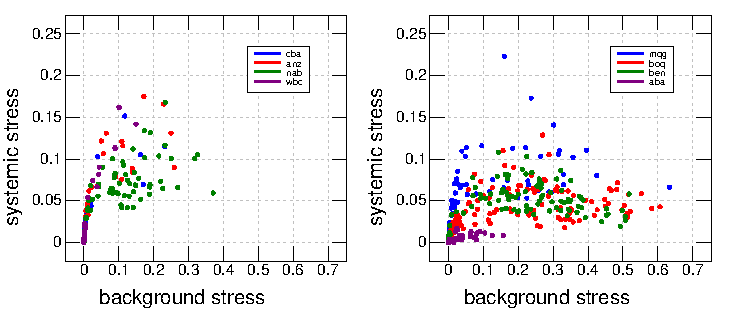
\includegraphics{figures/sysstress.pdf}
\caption{Systemic, $s_{it}$, versus background $\mu_{it}$   for four major banks (left panel) and four minor banks (right panel)  for 144 months.}
\label{sysstress}
\end{center}
\end{figure}

\fref{sysstress} plots systemic stress versus volatility stress for the eight Australian banks of \tref{banks}.   Generally volatility stress is higher than systemic stress.

\subsection{Flexible  stress  functions}

The further modification made to the SRISK methodology of \cite{brownlees2015} is to generalise the ``cutoff" functional form for stressing.   With the latter, stressed expectations are conditional expectations given a specified cutoff point.    In \cite{brownlees2015} the cutoff is in absolute terms:  a 10\% fall in the market although this can varied.   The cutoff methodology does not make explicit allowance for market volatility:   an absolute 10\% reduction is  increasingly plausible  as volatility increases.   However  SRISK does not  make judgement as to the likelihood of the conditioning stress event.   Thus SRISK mixes in various  sources of risk in an imprecise manner and it will be difficult to determine the implications of SRISK readings.

 This argues for specifying conditional behaviour in percentile terms relative to the then applicable market conditions.  After all, current market volatility is known and there is a good reason to disentangle current market conditions from the evaluation of what is likely to happen if further stress arrives in the system.

Say something about the generalized functional forms $\phi$ as well as the fact that we have firmly embedded and/or aligned the methodology with more ad--hoc approaches to stress testing.


\section{Comparing SRISK for different firms (not sure)}

Suppose of interest is whether $\beta_{it}$ varies similarly  across firms as $\tau$ varies where $\tau$ is the threshold, $\kappa$, or some other parameter used to compute $\beta_{it}$. High correlation implies high systemic risk since firms are simultaneously affected.

Define $\eps_{it}\equiv(\phi-1)p_{it}$ and $\eps_{it}$ as the vector with components $\eps_{it}$.  Then $\E(\eps_{it}|\tau)=\sigma_\phi(\tau)\beta_{it}(\tau)$, the stress in firm $i$ at the given parameter setting $\tau$  and
$$
\cov\{\E(\eps_{it}|\tau)\}=\cov(\eps_{t})-\E\{\cov(\eps_{it}|\tau)\}\ ,
$$
is the covariance between stresses as $\tau$, the stress parameter varies.   Thus the covariances and correlations between firms as stress parameters vary can be computed from the covariability between the $\eps_{it}$ and the ...

\begin{comment}
\subsection{Weihao - Allocating the market put}

The overall market shortfall after allowing for diversification between firms is
$$
p_{mt}\equiv k_+ |1-\e^{-\ell^*_{mt}+\nu_{mt}}|^+
= k_+|\Ex (1-\e^{-\ell^*_{it}+\nu_{it}})|^+
=I(\nu_{mt}<\ell_{mt}^*)k_+\Ex(1-\e^{-\ell^*_{it}+\nu_{it}}) 
$$
and hence the portion attributable to firm $i$ is $k_i(1-\e^{-\ell^*_{it}+\nu_{it}}) I(\nu_{mt}<\ell_{mt}^*)$, its capital shortfall or surplus when the overall market is in a shortfall. The allocation of the stressed expectation $\E(p_{mt})$ is then
$$
k_i\E\{(1-\e^{-\ell^*_{it}+\nu_{it}}) I(\nu_{mt}<\ell_{mt}^*)\}
$$
and applying $\Ex$ to the above expression yields $\E(p_{mt})$.
\end{comment}




\appendix
\renewcommand*{\thesection}{\Alph{section}}

\section{GARCH--DCC model}\label{garchdcc}

Denote the daily (log) return for firm $i$ at time $t$ as
\newcommand{\vareps}{\varepsilon}
\be{mean.model}
\delta_{it}=\mu_i+\sigma_{it}\eps_{it}\cq \eps_{it}\sim (0,1)\ ,
\ee
The volatility $\sigma_{it}$ is modelled as
\be{vol}
\sigma_{i,t+1}^2 = \omega+ \sigma^2_{it}\{\beta+(\alpha+\gamma \eps^-_{it})\eps_{it}^2\}  \cq  \eps^-_{it}\equiv I(\eps_{it}<0)=I(\delta_{it}<\mu)\ .
\ee
where $I$ denotes the indicator function.  Hence the response of $\sigma_{i,t+1}^2$ to $\eps_{it}^2$  is increased by $\gamma$   if
the rate of return is below the average $\mu_i$, compared to the response if $\delta_{it}>\mu_i$.  Equations \eref{mean.model} and \eref{vol} defined a simple threshold GARCH model:  called the TARCH(1,1).   In \eref{mean.model} the mean $\mu_i$ does not vary with time $t$ and in \eref{vol} it is assumed the terms  $\sigma_{it}^2$ and $\eps_{it}$ in the right hand side of \eref{vol} are sufficient to structure the dynamics of volatility. 

The model defined by \eref{mean.model} and \eref{vol} is estimated  for each security $i$ jointly with  a similar model for  the market,  $i=m$.   The correlations between securities and the market are modelled using  positive definite recursions   \citep{engle2002dynamic}
$$
(Q_{i,t+1}-S) = \alpha (\eta_{it}\eta_{it}'-S) + \beta (Q_{it}-S)\cq \eta_{it}\equiv(\eps_{it},\eps_{mt})' .
$$
Correlations $\rho_{it}$ recovered from the $Q_{it}$ are used as the correlation between $\eps_{it}$ and $\eps_{mt}$.

\section{Computations}

All model fits in this paper have been performed with the R language \citep{R-Development-Core-Team:2008aa} and in particular the rmgarch package described by \cite{ghalanos2012rmgarch}.  All other calculations were performed using the J language \citep{iverson2003j}.

In the forward simulated forward projections the  innovations are chosen randomly from past innovations.   These past innovations are chosen consistently:  at a particular $t$ either all or none of $\eps_{it}$ are chosen.

\section{Proof of system put is less   than debt weighted average put}\label{proof}

$$
1-\e^{-\ell_{it}} = \frac{ \kappa d_{it} - (1-\kappa)w_{it}}{\kappa d_{it}}\cq \Ex_d (1-\e^{-\ell_{it}}) = \frac{\kappa d_t - (1-\kappa) w_t}{\kappa d_t} = 1-\e^{-\ell_t} \ ,
$$
and similarly if $-\ell_{it}$ is replaced by $\nu_{it}-\ell_{it}$.   Hence 
$$
p_t\equiv |1-\e^{-\ell_t}|^+ \le \Ex_d (|1-\e^{-\ell_{it}}|^+)\equiv \overline p_t\ . 
$$ 

\section{Use of more general puts}

Consider the put $p_{it}(1+cp_{it})=p_{it}+cp_{it}^2 $ for some constant $c\ge 0$.   This put is zero if $p_{it}=0$ and has slope $1+2cp_{it}$ for $p_{it}>0$ and $p_{it}(1+cp_{it})>p_{it}$ if the put is positive.  Larger slopes $c$ imply greater payoff.  

The put $p_{it}+cp_{it}^2$ imposes a higher cost structure on defaults.    For every extra dollar of default the cost increases by $1+2cp_{it}$.   Further the stressed put value is
$$
\E(p_{it})\left\{1+c\E(p_{it})\right\} +c\left\{\cov(p_{it})\right\}+ \cov(p_{it},\phi) + c\left\{\cov(p^2_{it},\phi)\right\}
$$
$$
=\E(p_{it})\left\{1+c\E(p_{it})\right\} +c\left\{\cov(p_{it})\right\}+ \cov(p_{it}+cp^2_{it},\phi)\ .
$$
The first three terms in the final expression are unrelated to stress $\phi$: stress only impacts the last term. 

Can easily determine all terms via simulation.


\section{Data sources}\label{data}

(Geoff -- can you fill out?)



\section*{References}
\bibliography{/users/pietdejong/documents/research/srisk/piet2}

\end{document}
